% !TeX spellcheck = en_US
\documentclass[french]{yLectureNote}

\title{Introduction à la termodynamique}
\subtitle{Thermodynamique}
\author{Paulhenry Saux}
\date{\today}
\yLanguage{Français}

\professor{}

\usepackage{graphicx}%----pour mettre des images
\usepackage[utf8]{inputenc}%---encodage
\usepackage{geometry}%---pour modifier les tailles et mettre a4paper
%\usepackage{awesomebox}%---pour les boites d'exercices, de pbq et de croquis ---d\'esactiv\'e pour les TP de PC
\usepackage{tikz}%---pour deiffner + d\'ependance de chemfig
\usepackage{tkz-tab}
\usepackage{tabularx}%---pour dimensionner automatiquement les tableaux avec variable X
\usepackage{awesomebox}%---Pour les boites info, danger et autres
\usepackage{menukeys}%---Pour deiffner les touches de Calculatrice
\usepackage{fancyhdr}%---pour les en-t\^ete personnalis\'ees
\usepackage{blindtext}%---pour les liens
\usepackage{hyperref}%---pour les liens (\`a mettre en dernier)
\usepackage{caption}%---pour la francisation de la l\'egende table vers Tableau
\usepackage{pifont}
\usepackage{array}%---pour les tableaux
\usepackage{lipsum}
\usepackage{yFlatTable}
\usepackage{multicol}
\newcommand{\Lim}[1]{\lim\limits_{\substack{#1}}\:}
\renewcommand{\vec}{\overrightarrow}
\newcommand{\bz}{\overline{z}}
\DeclareMathOperator{\card}{card}
\renewcommand{\vec}{\overrightarrow}
\newcommand{\N}[0]{\mathbb{N}}
\newcommand{\R}[0]{\mathbb{R}}
\newcommand{\C}[0]{\mathbb{C}}
\newcommand{\dd}[0]{\mathrm{d}}
\newcommand{\er}{\vec{e_{\rho}}}
\newcommand{\ep}{\vec{e_{\varphi}}}
\newcommand{\pip}{\pi^+}
\newcommand{\pim}{\pi^-}
\newcommand{\mv}{\mathcal{V}}
\DeclareMathOperator{\Div}{Div}
\newcommand{\rot}{\vec{\mathrm{rot}}}
\newcommand{\grad}{\vec{\mathrm{grad}}}
\begin{document}
\setcounter{chapter}{1}
\chapter{Travail des forces de pression}
\section{Énergie reçue par un système fermé sous forme de travail par des forces de surface}

\explanation{1}{L'intégrale du flux d'énergie qui traverse la frontière}

\begin{flalign*}
    W_{i\to f} &= \int_{t_i}^{t_f} \phi_{\partial \Omega, W}(t)\dd t\explain{1}{right}{0}{0.5}{}
\end{flalign*}
On a 
\explanation{2}{$\varphi$ est une densité de flux d'énergie mécanique}
\begin{flalign*}
    \phi(t) &=  \int_{\partial \Omega} \varphi(M, t)\dd S
\end{flalign*}
Donc $\varphi(M,t) \dd S\dd t$ est le travail infinitésimal sur une surface infinitésimale sur un temps infinitésimal.

On a 
\begin{flalign*}
    \varphi(M,t) \dd S\dd t &= \dd\vec{F}(M,t)\cdot \dd \vec{l}(M,t)\\
    \varphi(M,t)\dd S &= \dd \vec{F}(M,t) \cdot \vec{v_m}(M,t)\\
    \varphi(M,t) &= \vec{\tau}(M,t)\cdot \vec{v_m}(M,t)\\
\end{flalign*}
Donc 
$$W_{i\to f} \int_{t_i}^{t_f} \int_{\partial \Omega} \vec{\tau}(M,t)\cdot \vec{v_m}(M,t)\dd S\dd t$$
\section{Cas d'un fluide contenu dans un cylidnre indéformable}
On étudie le cas d'un cylindre contenu dans un cylindre indéformable fermé par un piston mobile sans frottement.

\warningInfo{Convetion de signe}{On compte positive l'énergie qui rentre, le travail fournit, dans le cas contraire, c'est négatif.}
On cherche l'expression de la contraite $\tau$, grandeur locale instantannée.

Cette contrainte est uniforme sur toute la surface du piston, donc $\tau$ n'est plus locale, donc $\vec{\tau(M,t)} = \vec{\tau(t)} $.

De plus, la vitesse locale du point M sur le piston est celle du piston, donc $\vec{v_m}(M,t) = \vec{v_m}(t)$.

On en déduit :

\explanation{a1}{Car toutes les autres frontières sont immobiles, donc intégre juste sur la surface}

\begin{flalign*}
    W &= \int_{t_i}^{t_f}\int_{\partial \Omega} \vec{\tau(t)}\cdot \vec{v_p}(t)\dd S\dd t\\
    &= \int_{t_i}^{t_f}\int_{\S_p} \vec{\tau(t)}\cdot \vec{v_p}(t)\dd S\dd t\explain{a1}{right}{0}{0.5}{}\\
    &= \int_{t_i}^{t_f}\vec{\tau(t)}\cdot \vec{v_p}(t) \int_{\S_p} \dd S\dd t\\
     &= \int_{t_i}^{t_f}\vec{\tau(t)}\cdot \vec{v_p}(t)S_p \dd t\\
      &= \int_{t_i}^{t_f}\vec{F_{P/\Omega}}\cdot \vec{v_p}(t)\dd t\\
\end{flalign*}
On change maintenant de système : on étudie le piston pour trouver l'expression de $\vec{F_{P/\Omega}}$

On applique le PFD au piston : On note le poids la force de volume : $\vec{P} = \vec{F_{vol}}$.
\begin{flalign*}
    \vec{F_{vol}}+\vec{F_{\Omega/P}} + \vec{F_{atm}} &= \frac{\dd }{\dd t}(m_p \vec{v_p})\\
    \vec{F_{vol}}-\vec{F_{P/\Omega}} + \vec{F_{atm}} = \frac{\dd }{\dd t}(m_p \vec{v_p})\\
    \vec{F_{P/\Omega}} = \vec{F_{vol}}  + \vec{F_{atm}} - \frac{\dd }{\dd t}(m_p \vec{v_p})\\
\end{flalign*}

On peut réécrire le travail reçu par le gaz :

\newpage


\explanation{a2}{Si la masse est contante, le dernier terme est nul. Elle ne vaudrait pas 0 si le grain de sable arrivait avec une énergie cinétique non nulle.}

\explanation{a4}{On généralise en mettant une force exercée par un opérateur}

\explanation{a3}{$P_{ext}$ correspond à tout ce qui s'applique sur le système sauf les forces d'inertie.}

\begin{flalign*}
    W &=\int_{t_i}^{t_f}\vec{F_{vol}}\cdot \vec{v_p}(t)\dd t + \int_{t_i}^{t_f}\vec{F_{atm/P}}\cdot \vec{v_p}(t)\dd t - \int_{t_i}^{t_f} \frac{\dd }{\dd t}(m_p \vec{v_p}) \cdot \vec{v_p}(t)\dd t\\
    &=\int_{t_i}^{t_f}\vec{F_{vol}}\cdot \vec{v_p}(t)\dd t + \int_{t_i}^{t_f}\vec{F_{atm/P}}\cdot \vec{v_p}(t)\dd t - \int_{i}^{f} \frac{\dd }{}(m_p \vec{v_p}) \cdot \vec{v_p}(t)\\
     &=\int_{t_i}^{t_f}\vec{F_{vol}}\cdot \vec{v_p}(t)\dd t + \int_{t_i}^{t_f}\vec{F_{atm/P}}\cdot \vec{v_p}(t)\dd t \explain{a2}{right}{0}{0.5}{} \\
     &= \int_{t_i}^{t_f}m_p\vec{g}\cdot \vec{v_p}(t)\dd t + \int_{t_i}^{t_f}P_{atm}\vec{S_p}\cdot \vec{v_p}(t)\dd t\\
     &= \int_{t_i}^{t_f}\frac{S_p}{S_p}m_p\vec{g}\cdot \vec{v_p}(t)\dd t + \int_{t_i}^{t_f}P_{atm}\vec{S_p}\cdot \vec{v_p}(t)\dd t\\
     &= -\int (P_{atm}+ \frac{m_p g}{S_p})\dd V\\
     &= -\int (P_{atm}+  \frac{F_{op}}{S_p} +\frac{m_p g}{S_p})\dd V \explain{a4}{right}{0}{0.5}{}\\
     &= \int_i^f -P_{ext} \dd V \explain{a3}{right}{0}{0.5}{}
\end{flalign*}
\checkInfo{Remarque}{

\begin{flalign*}
    \int_{v_0}^{v_0} - P_{ext} \dd V \neq 0
\end{flalign*}
en général.
}
\section{Exemples}
\subsection{Compression monotherme brusque d'un gaz parfait}
On prend un piston dans un cylindre avec des parois non adiabatiques.

On le met dans un thermostat puis on le compresse subitement dans ce meme thermostat.

Données : 
\begin{itemize}
    \item $m_p = 5kg$
    \item $P_{ext} = P_{atm}$
    \item $T_{ext} = 300 K$
    \item $n = 1mol$
    \item $V_f = \frac{V_i}{2}$
    \item $\varnothing = 20cm$
\end{itemize}
Calculer $W_{i\to f}$.

À l'état initial :
\begin{itemize}
    \item $T_i = 300 K$
    \item $P_i = P_{atm} + \frac{m_p g}{S_p} = 10^5+1226$
    \item $V_i = \frac{nRT_i}{P_i} = 24.6\cdot 10^{-3}m^3$
\end{itemize}
À l'état final :
\begin{itemize}
    \item $T_f = 300 K$
    \item $V_f = 12.3\cdot 10^{-3}m^3$
    \item $P_f = \frac{nRT_f}{V_f} = 2\frac{nRt_i}{V_i} = 2P_i$
    \item $m_p' = (P_f-P_{atm})\frac{S_p}{g}$ car $P_f = P_{ext} = P_{atm} + \frac{m_p'g}{S_p}$
\end{itemize}
On cherche maintenant la travail :
\begin{flalign*}
    W_{i\to f}  &= -\int P_{ext}\dd V\\
&= -\int P_{atm}+ \frac{m_p'g}{S_p}\dd V\\
&= -P_f(v_f-V_i)
&= 2480 J
\end{flalign*}

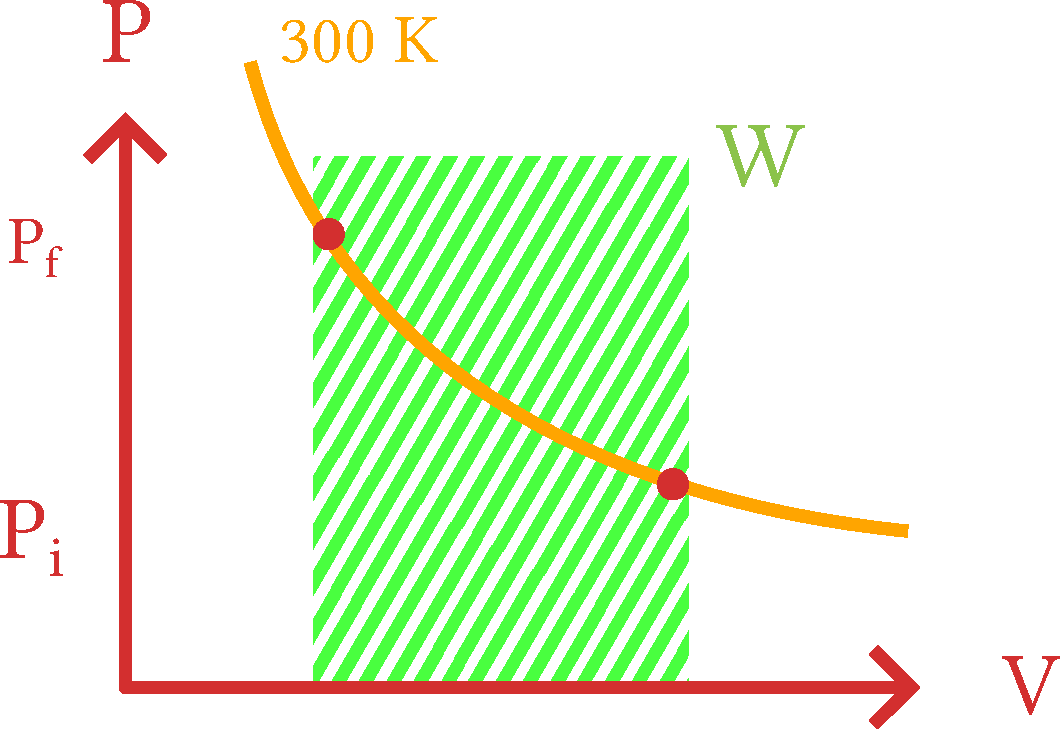
\includegraphics[scale=0.5]{clapeyron.pdf}

\subsection{Meme expérience de  façon quasi-statique}
On cherche maintenant la travail :
\newpage

\explanation{a5}{Il y a égalité car la transormation est quasi-statique, la pression extéieure est toujours égale à celle du système}

\begin{flalign*}
    W_{i\to f}'  &= -\int P_{ext}'\dd V\\
&= \int_i^f -p\dd v\explain{a5}{right}{0}{0.5}{}\\
&= -\int_i^f \frac{nRT}{V}\dd V\\
&= -nRT_{ext}\int \frac{1}{V}\dd V\\
&= nRT_{ext} \ln(2)
\end{flalign*}
\chapter{Principe de conservation de l'énergie}
On étudie un système fermé.
\section{Énoncé}
\begin{theorem}[Principe de conservation de Lavoisier]
    L'énergie est une grandeur conservative, elle ne peut \^etre ni crée, ni détruite.
\end{theorem}
\begin{theorem}[Deuxième définition]
    L'énergie d'un système isolé est une constante. L'énergie de l'univers est constante.
\end{theorem}
L'énergie de l'univers est notée $E_0$. C'est une grandeur extensive, donc $E_{\Omega}+E_{\bar{\Omega} = E_0}$.

On dérive par rapport au temps :
$$\frac{\dd E_{\Omega}}{\dd t}= -\frac{\dd E_{\bar{\Omega}}}{\dd t}$$

Pour que ce transfert soit instantanné, il faut que cela se passe à la frontière\marginTips{On appelle cela le principe de localité}.

$\frac{\dd E_{\Omega}}{\dd t}$ ne dépend que de $t$, qui est un flux, $\varphi_{\partial \Omega}$.

Donc 
\begin{theorem}[Principe de conservation de l'énergie]
    $\frac{\dd E_{\Omega}}{\dd t} = \varphi_{\partial \Omega}$
\end{theorem}
\section{Premier principe de la thermodynamique}
\subsection{Nature de l'énergie et des échanges d'énergie}
$$E_{\Omega} = E_{C} + E_p + U$$ avec $E_c$ l'énergie cinétique macroscopique en étudiant le centre de masse.
$\varphi_{\partial \Omega}$ est un flux d'énergie en Whatt, Joules/s.

$$\phi_{\partial \Omega} = \phi_{\partial \Omega, W} + \phi_{\partial \Omega, Q}$$
\begin{definition}[Flux d'énergie]
    On appelle flux d'énergie sous forme de chaleur tous les flux d'énergie qui ne
    sont pas mécaniques, i.e. liés au mouvement de la frontière.
\end{definition}
\subsection{Énoncé du premier principe}
On a $$\dd (E_c+E_p+U) = \phi_Q\dd t+\phi_W \dd t$$
En posant l'intégrale :
$$\int_i^f \dd (E_c+E_p+U) = \int_i^f \phi_Q\dd t+ \int_i^f\phi_W \dd t$$

En réérivant :
$$\Delta_{if} (E_c+E_p+U) = W_{i \to f} + Q_{i\to f}$$

\begin{theorem}[Énoncé du premier principe]
    $$\Delta_{if} (E_c+E_p+U) = W_{i \to f} + Q_{i\to f}$$
\end{theorem}
\criticalInfo{Utilité}{On ne s'en sert que pour calculer Q}
\section{Capacités thermiques}
\begin{definition}[Capacité thermique]
    La petite quantité d'énergie, notée $c$ qu'il faut fournir sous forme de chaleur pour augmenter sa temérature de $\dd T$:
    $$\delta Q = C\dd T$$
\end{definition}
\subsection{Capacité thermique à volume constant}
Elle est notée $c_v$.

On peut exprimer l'énergie interne du système : $U(T, V)$. On a alors :
$$\dd U = \frac{\partial U}{\partial T}\dd T + \frac{\partial U}{\partial V}\dd V$$ Comme
le volume est constant, on a $$\dd U = \frac{\partial U}{\partial T}$$

De plus, $$\dd U = \delta w + \delta Q = \delta Q = C_v \dd T$$.

On en déduit que
\begin{theorem}[Expression de la capacité thermique volume constant]
    $C_v = (\frac{\partial U}{\partial T})_V$.
\end{theorem}
\subsection{Capacité thermique à pression constante}
\subsubsection{Introduction}
Si la transormation est monobare, on a $$P_{ext} = Cst = p_i = p_f$$
On a 
\begin{flalign*}
    Q &= \Delta U - W\\
    &=\Delta U - \int - P_{ext}\dd V\\
    &= \Delta U + P_{ext}\Delta v
    &= U_f + P_{ext}V_f - (U_i+P_{ext}V_i)\\
    &= \Delta (U+pV)
\end{flalign*}
On pose $H = U+Pv$ qui est une fonction d'état extensive, notée Enthalpie. Elle correspond à la quantité de chaleur échangée sur une transformation monobare.

Si la transformation est monobare, on a $Q = \Delta H$
\begin{theorem}[Enthalpie]
    Notée $H = U+Pv$, elle permte d'écrire $Q = \Delta H$ pour une transformation monobare.
\end{theorem}
\subsubsection{Capacité}
On écrit :
\begin{flalign*}
    \dd H &= \frac{\partial H}{\partial T} \dd T + \frac{\partial H}{\partial P}\dd P\\
    &=\delta Q = C_p \dd T
\end{flalign*}
\begin{theorem}[Expression de la capacité thermique pression constante]
    $C_p = (\frac{\partial H}{\partial T})_P$.
\end{theorem}
\section{Phénoménologie}
\subsection{Incompressible}
Le volume est constant, par exemple l'eau liquide et les solides. On a donc $V = Cst$

De plus, $\dd U = C_v \dd T + \frac{\partial U}{\partial V}\dd V \Rightarrow U = C_v T+Cst$
L'énergie interne est proportionelle à la température
\subsection{Gaz parfaits}
On a $pV = nRT$ ou $pV = mrT$ ou $ p = \rho rT$ avec $r=\frac{R}{M}$
\begin{theorem}[Première loi de Joule]
    $U = U(T)$
\end{theorem}
Donc $\dd U = C_v \dd T + \frac{\partial U}{\partial V}\dd V \Rightarrow U = C_v T + Cst$
\subsection{Gaz réel}
On a $$p+\frac{n^2a}{V^2}(V-nb) = nRT$$

On a alors $U(T) = C_VT - \frac{n^2a}{V}+Cst$.
\section{Applications aux gaz parfaits}
\subsection{Relation de Mayer}
On a : 
\begin{flalign*}
    \dd U &= C_V \dd T\\
    \dd H &= \dd(U+pV)\\
    &= \dd U+\dd(pV)\\
    &= C_p \dd T + \frac{\partial H}{\partial P}= C_p \dd T
\end{flalign*}
\begin{theorem}[Relation de Mayer]
    $$C_p-C_v = nR$$
\end{theorem}
Posons maintenant $\gamma = \frac{C_p}{C_v}$. Il est connu la plupart du temps.
\begin{theorem}[Expression de Gamma]
    $$\gamma = \frac{C_P}{C_V}$$
\end{theorem}
\warningInfo{Résolution du système}{On en déduit $C_V = \frac{nR}{\gamma-1}$ et $C_p = \frac{nR\gamma}{\gamma-1}$}
\subsection{Relation de Laplace}
\criticalInfo{Hypothèses nécessaires}{
    \begin{itemize}
        \item Gaz parfait
        \item Transformation adiabatique (sans échange de chaleur avec le milieu extérieur = parois imperméables )
        \item Transformation quasi-statique
    \end{itemize}
}
\begin{theorem}[Relation de Laplace]
    $$TV^{\gamma-1} = K$$ ou $pV^\gamma = K'$ ou $p^{1-\gamma}T^\gamma=K''$.
\end{theorem}
\subsubsection{Exemple}
\begin{itemize}
    \item $P_i = 10^5 Pa$
    \item $T_i = 300K$
\end{itemize}

\begin{itemize}
    \item $P_f = 10P_i$
    \item $T_f = ?$
\end{itemize}
La température augmente ou reste constante ? Oui elle augmente meme si on ne chauffe pas.

On cherche a calculer $T_f$. On prend $\gamma = \frac{7}{5}$. On est dans le cas d'une compression quasi-statique de l'air.

On utilise les expressions 579K. On utilise la relation de contrainte, d'invariance $p^{1-\gamma}T^\gamma=K''$.

On veut maintenant le travail :
\begin{flalign*}
    W_{i\to f} &= \int -P_{ext}\dd V  = \int-p\dd V\\
    &= \int -\frac{nRT}{V}\dd V\\
    &= \int -\frac{Cst}{V^\gamma} = -Cst \frac{1}{\gamma+1}[V^{-\gamma+1}]^f_i\\
    &= \frac{\Delta(pV)}{\gamma-1}
\end{flalign*}
On peut aussi écrire $\Delta U = C_v(T_f-T_i) = W_{i\to f} = \frac{NR}{\gamma-1}(T_f-T_i)$
\subsection{Comparaison entre isotherme et adiabatique QS}
Isotherme : Pour maintenir lz gaz à la m\^eme chaleur, il faut enlever de la chaleur, donc les parois ne sont pas isolées.

Pour une compression adiabatique QS, $Q=0, W>0, \Delta U = C_v \Delta T >0$.

On calcule 
\begin{itemize}
    \item $\frac{\partial p}{\partial V}_T = -\frac{p}{V}$
    \item $\frac{\partial p}{\partial V}_{adia-QS} = - \gamma \frac{P}{V}$
\end{itemize}
On remarque que la pente de l'hyperbole de la transformation adiabatiqe vaut celle de l'isotherme multipliée par $\gamma$.
\section{Deux expériences}
\subsection{Détente de Joules et Gay Lussac}
On a 2 contenants isolés thermiquement. Ils sont séparés par un robinet. L'un est vide.
On ouvre le robinet.
La détente est adiabatique. En effet, $\Delta U = W + Q = C_v(T_1-T_0) = 0$
Cela vaut 0 car on est dans le vide.
\subsection{Détente de Joules-Thomson}
On appelle 1 les propriétés en amont du corps poreux et 2 celles en aval.

La détente est isenthalpique.
\chapter{Second principe de thermodynamique}
\section{Nécessité d'un second principe}
Expérience : On prend 2 compartiments rigides indéformables séparées par une paroi perméable à la chaleur.

On étudie la température. Le principe donne 
$$\Delta U^A = W^A+Q^A = Q^A$$ car parois fixes. De même pour le compartiment B:
$$\Delta U^B = Q^B$$
On a aussi $\Delta U^{A+B}=0 \Delta U^A+\Delta U^B \Rightarrow Q^A = -Q^B$
\begin{theorem}[Énoncé de Closus]
    La chaleur ne peut pas passer spontanement d'un corps froid à un corps chaud
\end{theorem}
\section{Cycle de Carnot(ditherme)}
2 adiabatiques Quasi-statique + 2 isothermes QS
$$\epsilon_{mot} \geq \epsilon_{mot, QS}$$L'efficacité est maximale si le cycle est entièrement quasi-statique.
\begin{definition}[Efficacité]
    $\epsilon = |\frac{Énergie utile}{Énergie couteuse}|$
\end{definition}
Donc $\epsilon_{mot} = \Big|\frac{W_{cycle}}{Q_chaud}\Big|$

On a $W_{cycle} + Q_{cycle} = Delta U_{cycle} = 0$

$W_{cycle} = - Q_{cycle} = -(Q_{ch} + Q_{fr})$ Ce sont les quantité de chaleur reçues.

$\epsilon = 1+ \frac{Q_{fr}}{Q_{chaud}}$ pour un moteur réel

Pour un moteur réel : $\epsilon_{max} = 1+\frac{Q_{fr,C}}{Q_{ch, C}}$

On cherche le travail sur un cycle.
$Q_{AB} = 0, Q_{BC} = -W_{BC} = + nRT_{chaud}\ln(\frac{V_C}{V_B}), Q_{CD} = 0, Q_{DA} = + nRT_{chaud}\ln(\frac{V_A}{V_D})$


On a donc $\epsilon_{max} = 1+ \frac{nR T_{fr}\ln(V_a/V_D)}{nRT_{ch}\ln(V_c/V_B)}$

En utilisant les relations de Laplace, on obtient : $\frac{V_c}{V_B} = \frac{V_d}{V_a}$.

On a donc $\epsilon_{max} = 1-\frac{T_F}{T_c}$

On obtient $\frac{Q_C}{T_c}+\frac{Q_F}{T_F}\leq 0$. C'est l'inégalité de Clausius.
\section{Cycle quelconque (toujours QS)}
$$\int \frac{\delta Q}{T}\leq 0$$ qui est l'intégrale de Clausius.
\subsection{Exemple}
On va de A vers B par 2 chemins différents Quasi-statique
Donc $\int_A^B \frac{\delta Q^{(1)}}{T}+\int_B^A\frac{\delta Q^{(2)}}{T} = 0$
On en déduit
\begin{theorem}
    $$\int_A^B \frac{\delta Q^{(1)}}{T} = \frac{\delta Q^{(2)}}{T}$$
\end{theorem}
Cela correspond donc à la variation d'une fonction d'état. L'intégrale est indépendant de la valeur du chemin.

On intriduit donc une fonction d'état , notée S appellée entropie.

On a donc $\Delta S_{AB} = \int_A^B \frac{\delta Q_{QS}}{T}$.

Cas avec un chemin non quasi-statique.
$$\int_A^B \frac{\delta Q}{T} < \int_A^B \frac{\delta Q_{qs}}{T} = Delta S_{AB}$$
Le premier terme est appellé terme d'échange d'entropie. L'échange est plus petit que la variation.
\end{document}


